% The PSBD decision for 1 input, from k perturbed passes to the verdict, with the
% calibration that runs once per model on the clean validation split. Symbols
% follow defenses/scores.py and defenses/decision.py. Compiled by render.py.
\documentclass[tikz,border=6pt]{standalone}
\usepackage[T1]{fontenc}
\usepackage{lmodern}
\usepackage{amsmath,amssymb}
\usetikzlibrary{arrows.meta,positioning,fit,backgrounds,calc}

\definecolor{tm}{HTML}{009E73}
\definecolor{rd}{HTML}{D55E00}
\definecolor{other}{HTML}{0072B2}
\definecolor{boxfill}{HTML}{F2F2F2}

\tikzset{
  stagebox/.style={draw, rounded corners=2pt, fill=boxfill, minimum height=13mm,
    text width=40mm, font=\footnotesize\sffamily, align=center},
  flow/.style={-{Stealth[length=2mm]}, thick},
  band/.style={draw=black!30, dashed, rounded corners=4pt, inner sep=6pt},
  bandlabel/.style={font=\footnotesize\sffamily\bfseries, anchor=south west},
}

\begin{document}
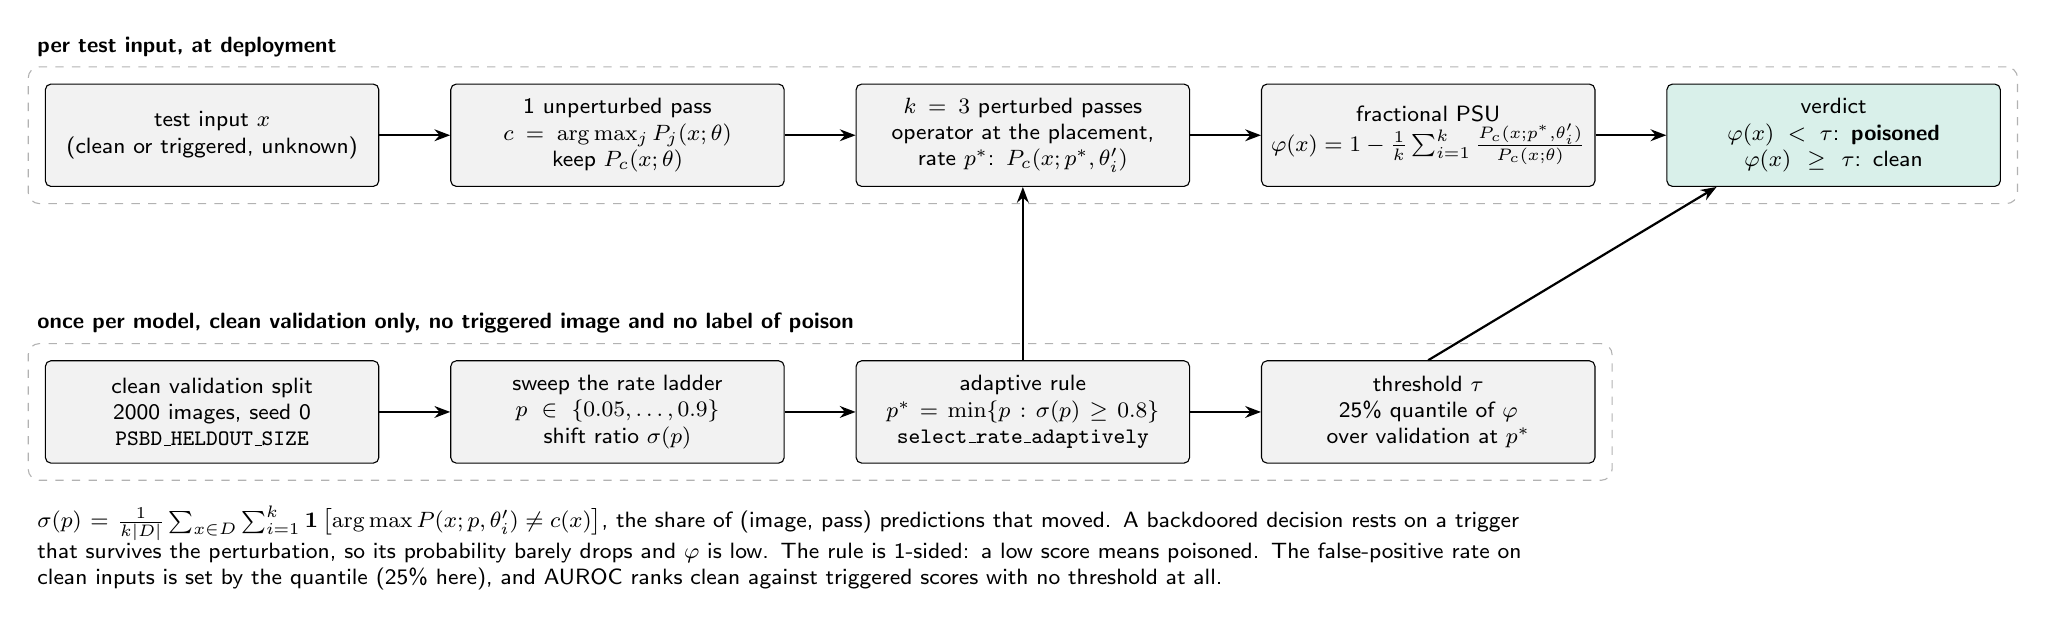
\begin{tikzpicture}[node distance=9mm]

% Per input.
\node[stagebox] (x) {test input $x$\\(clean or triggered, unknown)};
\node[stagebox, right=of x] (base) {1 unperturbed pass\\$c=\arg\max_j P_j(x;\theta)$\\keep $P_c(x;\theta)$};
\node[stagebox, right=of base] (passes) {$k=3$ perturbed passes\\operator at the placement,\\rate $p^\ast$: $P_c(x;p^\ast,\theta'_i)$};
\node[stagebox, right=of passes] (psu) {fractional PSU\\$\varphi(x)=1-\frac{1}{k}\sum_{i=1}^{k}\frac{P_c(x;p^\ast,\theta'_i)}{P_c(x;\theta)}$};
\node[stagebox, right=of psu, fill=tm!15] (verdict) {verdict\\$\varphi(x)<\tau$: \textbf{poisoned}\\$\varphi(x)\ge\tau$: clean};

\draw[flow] (x) -- (base);
\draw[flow] (base) -- (passes);
\draw[flow] (passes) -- (psu);
\draw[flow] (psu) -- (verdict);

% Once per model, on 2000 clean validation images.
\node[stagebox, below=22mm of x] (val) {clean validation split\\2000 images, seed 0\\\texttt{PSBD\_HELDOUT\_SIZE}};
\node[stagebox, right=of val] (ladder) {sweep the rate ladder\\$p\in\{0.05,\dots,0.9\}$\\shift ratio $\sigma(p)$};
\node[stagebox, right=of ladder] (rule) {adaptive rule\\$p^\ast=\min\{p:\sigma(p)\ge0.8\}$\\\texttt{select\_rate\_adaptively}};
\node[stagebox, right=of rule] (thr) {threshold $\tau$\\25\% quantile of $\varphi$\\over validation at $p^\ast$};

\draw[flow] (val) -- (ladder);
\draw[flow] (ladder) -- (rule);
\draw[flow] (rule) -- (thr);
\draw[flow] (rule.north) -- (passes.south);
\draw[flow] (thr.north) -- ($(verdict.south west)!0.3!(verdict.south)$);

\begin{scope}[on background layer]
  \node[band, fit=(x)(verdict)] (top) {};
  \node[band, fit=(val)(thr)] (bottom) {};
\end{scope}
\node[bandlabel] at (top.north west) {per test input, at deployment};
\node[bandlabel] at (bottom.north west) {once per model, clean validation only, no triggered image and no label of poison};

\node[font=\footnotesize\sffamily, align=left, anchor=north west, text width=190mm]
  at ($(bottom.south west)+(0,-2mm)$) {%
  $\sigma(p)=\frac{1}{k|D|}\sum_{x\in D}\sum_{i=1}^{k}\mathbf{1}\left[\arg\max P(x;p,\theta'_i)\ne c(x)\right]$, the share of (image, pass) predictions that moved. A backdoored decision rests on a trigger that survives the perturbation, so its probability barely drops and $\varphi$ is low. The rule is 1-sided: a low score means poisoned. The false-positive rate on clean inputs is set by the quantile (25\% here), and AUROC ranks clean against triggered scores with no threshold at all.};

\end{tikzpicture}
\end{document}
